\section{Methodology}
\label{sec:methodology}

This section describes the experimental methodology used to construct and evaluate Lightweight PC-STE. The study proceeds in six stages: (i) construction of a common one-second spectro-temporal representation across four vibration datasets; (ii) self-supervised initialization of the full PC-STE encoder; (iii) directionality-specific structural reduction to the K1 student; (iv) ensemble knowledge distillation under the frozen supervised training recipe; (v) a sealed matched Full-S1--K1 TEST comparison; and (vi) separate computational-efficiency and post-training Q8 deployment evaluations. The primary scientific comparison is Full-S1 versus K1; Q8 is explicitly secondary and was defined only after the primary study had been completed and frozen. Figure~\ref{fig:workflow} summarises the resulting pipeline and the points at which the protocol was frozen.

% Figure 1 — study workflow overview.
% Asset generated by scripts/publication_figures/fig01_workflow.py
\begin{figure}[tb]
  \centering
  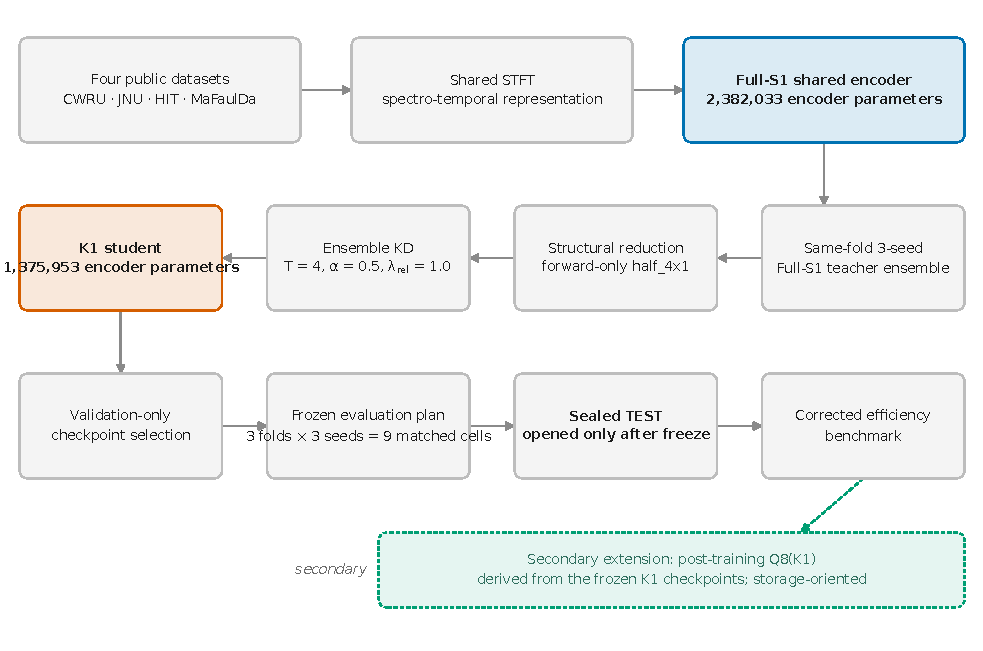
\includegraphics[width=\textwidth]{figures/fig01_workflow_overview.pdf}
  \caption{Overview of the frozen study workflow. One shared PC-STE encoder is
  trained across CWRU, JNU, HIT and MaFaulDa through a common spectro-temporal
  representation. The bidirectional Full-S1 encoder is structurally reduced to
  the forward-only K1 student, which is distilled from a same-fold ensemble of
  three independently seeded Full-S1 teachers. Checkpoints are selected on
  validation data only, and the sealed TEST partition was opened once, after the
  evaluation plan had been frozen. The post-training Q8(K1) stage (dashed) is a
  secondary, storage-oriented extension derived from the frozen K1 checkpoints
  and is not part of the primary comparison.}
  \label{fig:workflow}
\end{figure}


\subsection{Study Overview and Problem Formulation}
\label{subsec:overview}

Let $\mathcal{D}=\{\text{CWRU},\text{JNU},\text{HIT},\text{MaFaulDa}\}$ denote the four diagnostic datasets. A single encoder $E_{\theta}$ maps the representation of a vibration window to a global embedding $z\in\mathbb{R}^{192}$. Each dataset $d\in\mathcal{D}$ has a separate linear classification head $h_d$, so the encoder parameters are shared while the output label spaces remain dataset-specific:
\begin{equation}
    \hat{y}_d = h_d\!\left(E_{\theta}(x_d)\right).
\end{equation}
This design avoids forcing incompatible class taxonomies into one output head. CWRU, JNU, HIT, and MaFaulDa therefore contribute to a common representation while preserving their own labels.

Full-S1 is the reference model. It uses the full bidirectional PC-STE encoder initialized from masked-reconstruction self-supervision. K1 is the lightweight student. It retains the same embedding width, patch stem, coordinate encoder, four temporal stages, cross-band mixer, validity-aware pooling, and dataset-specific heads, but each bidirectional temporal layer is replaced by its forward-only counterpart. Q8(K1) is a deterministic post-training quantized representation of K1 and is evaluated as a secondary deployment extension.

\begin{table}[t]
\centering
\caption{Full-S1 and K1 architecture summary. The student preserves model width and temporal depth while removing the reverse state-space direction.}
\label{tab:model_architecture}
\small
\begin{tabular}{lcc}
\toprule
Property & Full-S1 & K1 \\
\midrule
Shared embedding width & 192 & 192 \\
Temporal stages & 4 & 4 \\
Directions per stage & 2 (forward + backward) & 1 (forward) \\
Mamba inner width & 384 & 384 \\
State dimension & 16 & 16 \\
Patch size (frequency $\times$ time) & $16\times8$ & $16\times8$ \\
Dataset-specific heads & 4 & 4 \\
Encoder parameters & 2,382,033 & 1,375,953 \\
Complete-model parameters & 2,385,893 & 1,379,813 \\
\bottomrule
\end{tabular}
\end{table}


The central hypothesis concerns retention rather than raw superiority: after structural reduction and distillation, K1 should not lose more than a prespecified amount of aggregate diagnostic performance relative to Full-S1. Computational measurements are conducted separately from the predictive evaluation so that inference efficiency cannot influence model selection.

\subsection{Datasets and Experimental Protocol}
\label{subsec:datasets}

The final study uses four public rotating-machinery datasets with different sampling rates, machinery configurations, and label spaces: CWRU~\citep{CWRUDataset}, JNU~\citep{JNUDataset}, HIT~\citep{Hou2023HIT}, and MaFaulDa~\citep{MaFaulDaDataset}. Table~\ref{tab:datasets} summarizes the role of each dataset. Raw signals remain at their native sampling rates; the final CWRU protocol uses official native 12~kHz recordings only and does not mix in the 48~kHz files. JNU and MaFaulDa are sampled at 50~kHz, while HIT is sampled at 25~kHz. Dataset source material is retained under the terms of the original providers.

\begin{table}[t]
\centering
\caption{Datasets and frozen evaluation principles used in the publication study. The protocols are designed to prevent direct window leakage but do not establish unseen-machine generalization.}
\label{tab:datasets}
\small
% ragged-right X columns: justified narrow cells produced visibly stretched
% inter-word gaps in the MaFaulDa row.
\begin{tabularx}{\textwidth}{l c c >{\raggedright\arraybackslash}X >{\raggedright\arraybackslash}X}
\toprule
Dataset & Classes & Native rate & Split principle & Scope of claim \\
\midrule
CWRU & 3 & 12 kHz & TRAIN: 0+1 hp; validation: 2 hp; TEST: 3 hp & Cross-load on the same rig, not cross-machine \\
JNU & 4 & 50 kHz & Guarded temporal split within frozen recordings & Held-out windows/segments, not unseen-machine \\
HIT & 3 & 25 kHz & Frozen logical-recording split & Held-out recordings under the registered protocol \\
MaFaulDa & 10 & 50 kHz & Grouped by configuration/severity & Held-out grouped conditions on the same simulator \\
\bottomrule
\end{tabularx}
\end{table}


All models operate on one-second windows. Training uses overlapping windows with a 0.5-s stride, while validation and TEST use a 1.0-s stride. The split definitions were frozen before the publication comparison. CWRU uses a load partition in which 0 and 1~hp form TRAIN, 2~hp forms validation, and 3~hp forms TEST. This evaluates cross-load behaviour on the same experimental rig; it is not an unseen-machine test. JNU uses a guarded temporal split within the available recordings, HIT uses a frozen logical-recording split rather than adopting an uncontrolled random window split, and MaFaulDa uses grouped assignments by machine configuration/severity. These protocols reduce direct window leakage, but none establishes transfer to a completely unseen machine or acquisition system. Accordingly, no cross-machine generalization claim is made.

The final design contains three global folds and three random seeds, $s\in\{42,1337,2026\}$, for nine matched cells. Within a cell $(f,s)$, Full-S1 and K1 are compared using the same fold definition and corresponding seed. TEST data are excluded from model training and validation-based checkpoint selection.

\subsection{Spectro-Temporal Input Representation}
\label{subsec:representation}

Each one-second vibration window is transformed to the frozen N2 magnitude short-time Fourier transform (STFT) representation. The transformation is performed at the dataset's native sampling rate and followed by a $\log(1+x)$ magnitude transform. The N2 configuration was selected before the final publication comparison and then held fixed. The representation stores both the spectral values and their physical frequency and time coordinates, allowing the same encoder to operate on grids arising from different native sampling rates without introducing a dataset-specific encoder branch.

Normalization is fitted on TRAIN only for every fold and dataset. The standard deviation denominator is lower-bounded by 0.05 to prevent unstable scaling of near-constant cells. The fitted normalizer is then frozen and reused for validation and TEST. When tensor completion is required for batching or patchification, padded cells are zero-filled and explicitly masked; no interpolation is used to fabricate unobserved frequency content.

PC-STE divides each spectrogram into $16\times8$ time--frequency patches. A patch stem applies a $3\times3$ convolution with eight channels and GELU activation inside each patch, followed by a linear projection to $d_{\mathrm{model}}=192$. The model additionally computes physical patch centres in kHz and seconds from valid cells only. Fourier coordinate features derived from these absolute physical coordinates are projected into the model width and added to the patch embeddings. Thus, positional information represents physical frequency and time rather than only grid indices.

\subsection{Full PC-STE and Self-Supervised Initialization}
\label{subsec:fullpcste}

The full encoder contains four temporal layers. Within each frequency band, patch tokens are processed along time by independently parameterized forward and backward Mamba blocks. For an input sequence $X$, one bidirectional layer can be written as
\begin{equation}
    Y = X + \frac{1}{2}\left[
    \mathcal{M}_{\mathrm{fwd}}(\mathrm{LN}(X)) +
    \mathrm{flip}\left(\mathcal{M}_{\mathrm{bwd}}(\mathrm{flip}(\mathrm{LN}(X)))\right)
    \right],
\end{equation}
where $\mathcal{M}$ is a Mamba-1 selective state-space block. In the implementation, $d_{\mathrm{inner}}=384$, $d_{\mathrm{state}}=16$, the depthwise causal convolution has width four, and the time-step projection rank is $\lceil192/16\rceil=12$. The official fused Mamba CUDA implementation was unavailable on the experimental software stack; therefore, the same Mamba-1 recurrence is executed in pure PyTorch. This changes implementation speed but not the model equations.

After the temporal backbone, valid tokens are averaged within each frequency band. An Hz-aware cross-band mixer computes data-dependent interactions using both the band summaries and their physical frequency features. Finally, validity-masked pooling across bands produces the shared 192-dimensional embedding consumed by the four dataset heads. The encoder has 2,382,033 trainable parameters; including the heads, the complete Full-S1 model contains 2,385,893 parameters.

Full-S1 is initialized through masked spectrogram reconstruction. During self-supervised training, 60\% of valid patches are selected by the frozen random-mask geometry and reconstruction loss is evaluated on the masked content. Training uses AdamW with learning rate $3\times10^{-4}$, betas $(0.9,0.95)$, weight decay 0.05, gradient clipping at global norm 1.0, five warm-up epochs, and cosine decay to $10^{-6}$. Self-supervised training runs for 60 epochs. The resulting encoder initializes the supervised Full-S1 models; downstream training uses the same optimizer family for 50 epochs, with validation-only checkpoint selection.

\subsection{K1 Structural Compression}
\label{subsec:k1}

K1 has the registered architecture name \texttt{half\_4x1}. The compression operation is deliberately narrow: each of the four bidirectional temporal layers is replaced by a forward-only layer while all four temporal stages are retained. If $F_l$ and $B_l$ denote the forward and backward Mamba blocks at layer $l$, Full-S1 uses both directions whereas K1 keeps $F_l$ only:
\begin{align}
  \text{Full-S1: } & X_{l+1}=X_l+\tfrac{1}{2}\left(F_l(\mathrm{LN}(X_l))+B_l^{\leftarrow}(\mathrm{LN}(X_l))\right), \\
  \text{K1: } & X_{l+1}=X_l+F_l(\mathrm{LN}(X_l)).
\end{align}
The registered residual convention is \texttt{mean\_of\_remaining}, which gives the retained branch unit residual scale rather than preserving the previous factor of one half.

K1 is constructed by deterministic surgery from the matched Full-S1 checkpoint in the same fold--seed cell. The patch stem, coordinate encoder, forward Mamba parameters, final temporal normalization, cross-band mixer, and dataset heads are copied from the teacher-side model; reverse-direction parameters are dropped. This produces a 1,375,953-parameter shared encoder and a 1,379,813-parameter complete model. Because the hidden width and number of temporal stages are unchanged, the comparison isolates directionality reduction more directly than a wholesale redesign of the student.

\subsection{Ensemble Knowledge Distillation}
\label{subsec:distillation}

For each fold $f$, the teacher set comprises the three independently seeded Full-S1 checkpoints from that fold:
\begin{equation}
  \mathcal{T}_f = \{T_{f,42},T_{f,1337},T_{f,2026}\}.
\end{equation}
Cross-fold teacher mixing is forbidden. Teacher inference is deterministic, and only TRAIN and validation outputs are cached for distillation; TEST outputs never enter K1 training.

For a dataset with class logits $z_k$ from teacher $k$, the classification soft target is the mean of the temperature-scaled teacher probabilities:
\begin{equation}
  \bar{p}_T = \frac{1}{3}\sum_{k=1}^{3}\mathrm{softmax}\left(\frac{z_k}{T}\right),
  \qquad T=4.
\end{equation}
The student classification loss combines hard-label cross-entropy and forward KL divergence from the ensemble target to the student distribution:
\begin{equation}
\mathcal{L}_{\mathrm{KD}}=
(1-\alpha)\,\mathcal{L}_{\mathrm{CE}}+
\alpha T^2\,D_{\mathrm{KL}}\!\left(\bar{p}_T\,\|\,p_s^T\right),
\qquad \alpha=0.5.
\end{equation}
A relational term aligns cross-band attention distributions between K1 and the same-cell Full-S1 teacher. Invalid or padded bands are excluded before the distributions are renormalized. The final registered loss adds this term with weight $\lambda_{\mathrm{rel}}=1.0$. Losses are first averaged over windows within each dataset and then averaged equally across datasets, ensuring that datasets with more windows do not dominate an optimization step.

K1 is trained for 50 epochs using the frozen AdamW recipe described above. The effective batch is 64 windows, organized as 16 windows per dataset. Checkpoint selection uses the maximum validation Macro-4 Macro-F1 (recorded in the frozen artifacts as \texttt{macro\_domain\_f1}) under strict improvement; exact ties retain the earlier epoch. There is no early stopping and no TEST-based model selection.

\subsection{Secondary Q8 Quantization Extension}
\label{subsec:q8}

Q8 is evaluated only after the Full-S1--K1 study and the primary efficiency benchmark were complete. It is therefore a secondary deployment extension rather than an arm of the original confirmatory comparison. Each of the nine frozen K1 \texttt{best.pt} checkpoints is converted deterministically, without retraining, fine-tuning, or calibration.

The registered accuracy representation applies per-output-channel symmetric 8-bit quantization to 23 allowlisted linear modules. For output channel $c$, the weight scale is
\begin{equation}
  s_c=\frac{\max_j |w_{c,j}|}{127}, \qquad
  q_{c,j}=\mathrm{clip}\left(\mathrm{round}(w_{c,j}/s_c),-127,127\right).
\end{equation}
The stored compact state retains the integer weights and scales, whereas evaluation of the registered \texttt{sim} representation dequantizes these weights to FP32 for computation. The time-step projection, state parameters $A_{\log}$ and $D$, depthwise convolution, layer normalizations, patch-stem convolution, and selective-scan recurrence remain FP32. Overall, 1,322,816 of 1,379,813 parameters (95.87\%) are stored as int8 weights in the quantized plan.

A separate \texttt{cpu\_dynamic} representation uses \texttt{torch.ao} dynamic quantization with the \texttt{fbgemm} backend, adding dynamic activation quantization for the same allowlisted linear layers. This is the CPU deployment representation used for runtime measurement. It is not numerically identical to \texttt{sim}; therefore, the Q8 TEST non-inferiority statement applies only to \texttt{sim}. The preserved implementation provides no true INT8 CUDA execution path, so no Q8 GPU latency or GPU-memory claim is made.

\subsection{Evaluation Metrics and Statistical Analysis}
\label{subsec:stats}

For each dataset, the evaluation records accuracy, balanced accuracy, macro precision, macro recall, Macro-F1, one-vs-rest Macro-AUC, classwise precision/recall/F1, and the confusion matrix. The primary publication endpoint is equal-domain Macro-4 Macro-F1,
\begin{equation}
  F_{\mathrm{M4}} = \frac{1}{4}\sum_{d\in\mathcal{D}}F_{1,d},
\end{equation}
so that every dataset contributes equally regardless of its number of windows. Macro-4 Macro-AUC is a secondary aggregate endpoint and is computed analogously when all four dataset AUC values are finite.

The experimental unit for the primary comparison is the matched fold--seed cell. For cell $i$, the paired difference is
\begin{equation}
  \Delta_i = F_{\mathrm{M4},i}^{\mathrm{K1}} - F_{\mathrm{M4},i}^{\mathrm{Full-S1}},
  \qquad i=1,\ldots,9.
\end{equation}
The largest acceptable Macro-F1 loss was fixed at $m=0.02$ before the final sealed TEST evaluation was run; it was not chosen after any TEST outcome had been observed. The non-inferiority hypothesis is
\begin{equation}
  H_0:\mathbb{E}[\Delta]\leq -m, \qquad
  H_1:\mathbb{E}[\Delta]>-m, \qquad m=0.02.
\end{equation}
The exact one-sided test is performed by first shifting each paired difference by the margin, $\Delta_i'=\Delta_i+m$, then enumerating all $2^9=512$ sign-flip patterns. Non-inferiority passes only when the exact one-sided $p$-value is below 0.05 and the observed shifted mean is positive. A two-sided exact superiority test is reported only after the non-inferiority gate passes, and is treated as supportive secondary evidence rather than the primary study claim. Descriptive dispersion is the sample standard deviation across all nine cells.

For Q8, the paired unit is again fold--seed, but the historical quantization margin is $-0.01$ and the contrast is Q8 minus K1. The exact one-sided sign-flip procedure is reused without adding a superiority test. Because the broader historical multiple-hypothesis family was not executable in the publication extension, the Q8 contrast is reported as a standalone secondary analysis without family-wise multiplicity adjustment.

\subsection{Computational Efficiency Evaluation}
\label{subsec:efficiency_method}

Model complexity is characterized by encoder and complete-model parameter counts, standardized FP32 state-dictionary size, FLOPs per one-second window, batch-1 latency, batch-32 throughput, and GPU peak allocated memory. FLOPs combine a dense-operator count with an analytic selective-scan term; the same convention is applied to both Full-S1 and K1. Because CWRU uses a smaller native-12~kHz spectrogram grid than the historical mixed-rate implementation, the scan term uses the final publication representation rather than the superseded mixed-rate band count.

Runtime measurement uses one deterministically fixed representative pair, global fold 1 / seed 42, selected by the rule ``lowest fold, then lowest seed'' before any efficiency outcome was observed. The first validation window in frozen manifest order is used for each dataset, and the same inputs are supplied to both models. Measurements were obtained on an idle Intel Core i9-14900 host with an NVIDIA RTX 4000 Ada Generation GPU, PyTorch 2.12.0+cu130, and CUDA 13.0. CPU timing uses one thread.

The authoritative timing correction runs both models in evaluation mode with PyTorch inference mode explicitly verified inside the timed loop. CPU batch-1 measurements use 100 warm-up and 1000 timed iterations per dataset and scope; GPU batch-1 uses 200 warm-up and 1000 timed iterations with synchronization. Model-only latency measures prepared representation to logits, while end-to-end latency additionally includes STFT construction and normalization but excludes disk I/O. Batch-32 throughput is measured separately. Full-S1 and K1 are interleaved to reduce temporal bias, and the headline value is the equal-domain mean of the four per-dataset medians. All latency measurements use the pure-PyTorch selective scan rather than a fused Mamba kernel, so absolute times should be interpreted for this software stack rather than as hardware-independent constants.
